\appendix
\onecolumn
\section{Matheron updates}\label{app:matheron}
The pathwise Gaussian process update (\emph{Matheron update}), credited to unpublished works of Matheron~\citep{WilsonPathwise2021,DoucetNote2010} is a method of simulating from a conditional of some jointly Gaussian variate.
The Matheron update \(\pi\) for a partitioned Gaussian random vector
\(\begin{bmatrix} \vrv{y} &\vrv{w}
\end{bmatrix}^{\top}\) is a mapping
\begin{align*}
\pi: \left(\vv{y},\vv{w};\Law\left(\begin{bmatrix}\vrv{y}\\\vrv{w}\end{bmatrix}\right) \right)\mapsto \vv{y}' 
\end{align*}
such that
\begin{align*}
\begin{bmatrix}\vrv{y}\\\vrv{w}\end{bmatrix}&\sim \Law\left(\begin{bmatrix}\vrv{y}\\\vrv{w}\end{bmatrix}\right) \\
&\Rightarrow\\
\pi\left(\vrv{y},\vv{w};\Law\left(\begin{bmatrix}\vrv{y}\\\vrv{w}\end{bmatrix}\right) \right) &\stackrel{d}{=}  \vrv{y}\gvn (\vrv{w}{=}\vv{w}) .\numberthis\label{eq:matheron-prop}
\end{align*}
Where the joint distribution of the random variates is clear from context we suppress the third argument of the function \(\pi\).
\russ{In the last equation (not first), there are three typesettings $\vrv{w}, w$ and $\vv{w}$, but I think we only need 2, right? $\vrv{w}$ and $w$?}\danm{yes, we have alternated between \(\vv{w}\) and \(w\) throughout this whole document; that needs fixing everywhere. I think dan P has been standardising on \(\vv{w}\)} \russ{Also shouldn't $\pi$ have 3 arguments, because it accepts both $\vrv{w}$ and $w$ as an input?} \danm{oh yeah it should, I mean, depending on how we wish to phrase; the distributions could be absorbed into \(\pi\). it should act on two distributions ( a joint distribution, really) and an observation. How does current phrasing look? Other thought, though: we are already doing a non-standard presentation of the update rule; should we save this weird phrasing for some future paper where we exploit the generality?}

Such a rule is known for Gaussian RVs \begin{align*}
    \begin{bmatrix}\vrv{y}\\ \vrv{w}
\end{bmatrix}\sim\mathcal{N}\left(\begin{bmatrix}
    m_{\vrv{y}}\\ m_{\vrv{w}}
\end{bmatrix},\begin{bmatrix}
    \mm{K}_{\vrv{y}\vrv{y}} & \mm{K}_{\vrv{y}\vrv{w}} \\
    \mm{K}_{\vrv{w}\vrv{y}} & \mm{K}_{\vrv{w}\vrv{w}}
\end{bmatrix}\right).
\end{align*}
Since these variates are jointly Gaussian, the conditional is also Gaussian and a necessary and sufficient condition for the update rule may be written in terms of the first two moments of the conditional as
\begin{align*}
    %\Ex [\pi(\vrv{y},\vv{w}) )]
    %&=
    \Ex[\vrv{y}\gvn \vrv{w}{=}w] 
    &=m_{\vrv{y}}
        +\mm{K}_{\vrv{w}\vrv{y}} \mm{K}_{\vrv{w}\vrv{w}}^{-1}(w-m_{\vrv{w}})  &\text{ first moment}\numberthis \label{eq:app-gaussian-cond-mean}\\
    %\var [\pi(\vrv{y},\vv{w}) )] 
    %&= 
    \var[\vrv{y}\gvn \vrv{w}{=}w] 
    &=\mm{K}_{\vrv{y}\vrv{y}} 
        -\mm{K}_{\vrv{w}\vrv{y}} \mm{K}_{\vrv{w}\vrv{w}}^{-1}\mm{K}_{\vrv{y}\vrv{w}}. &\text{ second moment}\numberthis \label{eq:app-gaussian-cond-var}
\end{align*}
The Gaussian Matheron update which satisfies \eqref{eq:matheron-prop} is
\begin{align*}
\pi: \left(\vv{y},\vv{w};\mathcal{N}\left(\begin{bmatrix}
    m_{\vrv{y}}\\ m_{\vrv{w}}
\end{bmatrix},\begin{bmatrix}
    \mm{K}_{\vrv{y}\vrv{y}} & \mm{K}_{\vrv{y}\vrv{w}} \\
    \mm{K}_{\vrv{w}\vrv{y}} & \mm{K}_{\vrv{w}\vrv{w}}
\end{bmatrix}\right)\right) \mapsto 
\vv{y}+\mm{K}_{\vrv{w}\vrv{y}} \mm{K}_{\vrv{w}\vrv{w}}^{-1}\left[\vv{w}-\vrv{w}\right].\numberthis\label{eq:pathwise-update-disc-app}
\end{align*}
\russ{I think this should be 3 argument version, as above? In particular, it should not involve ${m}_{\vrv{w}}$. }\danm{certainly should not; updated. Although this notation still feels not quite right. are we `covertly' randomising over \(\vrv{w}\)? or is it plain enough? }
Note that this update does not require us to calculate \(\mm{K}_{\vrv{y}\vrv{y}}\)
and further, may be conducted without needing to evaluate the density of the observation.

The Matheron update is used, for example, in~\citep{WilsonEfficiently2020} for the case that we have a Gaussian observation operator \(\op{T}: \vrv{y} \mapsto \mm{T}\vrv{y} + \vv{b} + \vrv{z}\) with \(\mm{T}\) linear, \(\vv{b}\) deterministic, and \(\vrv{z}\sim\mathcal{N}(0,\mm{K}_{\vrv{z}})\), resulting in joint distribution
\begin{align*}
\begin{bmatrix}
\vrv{y}\\ \vrv{w}
\end{bmatrix} =
\begin{bmatrix}
\vrv{y}\\ \mm{T}\vrv{y} + \vv{b} + \vrv{z}
\end{bmatrix}\sim\mathcal{N}\left(
\begin{bmatrix}
    m_{\vrv{y}}\\ \mm{T}m_{\vrv{y}} + \vv{b}
\end{bmatrix},\begin{bmatrix}
    \mm{K}_{\vrv{y}\vrv{y}} & \mm{K}_{\vrv{y}\vrv{y}}\mm{T}^{\top} \\
    \mm{T}\mm{K}_{\vrv{y}\vrv{y}} & \mm{T}\mm{K}_{\vrv{y}\vrv{y}}\mm{T}^{\top}+\mm{K}_{\vrv{z}}
\end{bmatrix}\right).
\end{align*}
In such cases, \eqref{eq:pathwise-update-disc-app} becomes
\begin{align*}
\pi(\vv{y},\vv{w})
&=\vrv{y}+\mm{T}\mm{K}_{\vrv{y}\vrv{y}} \left(\mm{T}\mm{K}_{\vrv{y}\vrv{y}}\mm{T}^{\top}+\mm{K}_{\vrv{z}}\right)^{-1}\left[\vv{w}-\mm{T}m_{\vrv{y}}-\vv{b}\right].\numberthis\label{eq:matheron-linear-obs}
\end{align*}

% \russ{I don't understand the motivation for this. If I understand correctly, Matheron update is a solution to an optimisation problem. This optimisation problem is not ``linear least squares'' in the traditional sense, since it involves just matching the coordinates of the vector, not solving a linear system. In this sense, it is trivial because any vector $b$ admits a representation $b = \argmin_a \Vert a - b \Vert^2$, or more generally $b = \argmin_a D(a,b)$ where $D$ is nonnegative and zero iff $a=b$.}
% \danm{You're right this does not add anything non-trivial. I was hoping that this would be neater than the previous version of this appendix, but this method is not The Way,}

In this work, we suppose that the joint distribution of \(\begin{bmatrix} \vrv{y} &\vrv{w}\end{bmatrix}^{\top}\) arises from a nonlinear, stochastic operator \(\op{T}\) such that \(\op{T}\vrv{y}=\vrv{w}\).
We want to construct an approximate analogue to the Matheron update which  updates the ensemble samples so that their empirical \emph{ensemble} statistics approximately satisfy \eqref{eq:app-gaussian-cond-mean} and \eqref{eq:app-gaussian-cond-var}.
We hope this can work if we generalise the basic Matheron rule in two senses:
\begin{enumerate}
    \item An ensemble version, which rather than acting upon the first 2 moments of our prior belief distribution, should act upon an \emph{ensemble of samples} drawn from the prior belief distribution, which is 
    \item applicable for nonlinear and stochastic \(\op{T}\)
\end{enumerate}
This is essentially the setting of the stochastic Ensemble Kalman filter~\citep{EvensenData2009} (EnKF).

Rewriting \eqref{eq:app-gaussian-cond-mean} and \eqref{eq:app-gaussian-cond-var} in terms of moments of this general \(\op{T}\vrv{y}=\vrv{w}\),
% If
% \(\Law(\vrv{y}')= \Law(\vrv{y}\gvn \vrv{w}{=}w)\) and moreover \(\op{T}\vrv{y}=\vrv{w}\) and they  were Gaussian rvs, 
% then we could completely characterise the relationship via
\begin{align*}
    \Ex [\vrv{y}']
    &= \Ex[\vrv{y}\gvn \op{T}\vrv{y}{=}w]\\
    &=\Ex[\vrv{y}]
        +\var[\vrv{y},\op{T}\vrv{y}] \var^{-1}[\op{T}\vrv{y},\op{T}\vrv{y}](w-\Ex[\op{T}\vrv{y}])  \numberthis \label{eq:app-gaussian-cond-mean-imp}\\
    \var [\vrv{y}'] 
    &= \var[\vrv{y}\gvn \op{T}\vrv{y}{=}w] \\
    &=\var[\vrv{y},\vrv{y}]
        -\var[\vrv{y},\op{T}\vrv{y}] \var^{-1}[\op{T}\vrv{y},\op{T}\vrv{y}]\var[\op{T}\vrv{y},\vrv{y}].\numberthis \label{eq:app-gaussian-cond-var-imp} 
\end{align*}
In the ensemble setting we maintain ensembles
\(\mm{Y}=\begin{bmatrix}\vv{y}^{(1)}& \cdots& \vv{y}^{(N)}\end{bmatrix}\) and
\(\mm{W}=\begin{bmatrix}\vv{w}^{(1)}& \cdots& \vv{w}^{(N)}\end{bmatrix}\) where 
\(\vv{w}^{(i)} \sim\op{T}\vv{y}^{(i)},i=1,\dots,N\), which we write \(\mm{W}=\op{T}{\mm{y}}\).
Further, we construct a mean estimate
\(\widehat{\Ex}[\vrv{y}]=\overline{\mm{Y}}=\frac1N\sum_{i=1}^N\vv{y}^{(i)}\)
and a variance estimate \(\widehat{\var}=\breve{\mm{Y}}\breve{\mm{Y}}^{\top}\) where
\(\breve{\mm{Y}}={\textstyle \frac{1}{\sqrt{N-1}}}\begin{bmatrix}\vv{y}^{(i)}-\overline{\mm{Y}}\end{bmatrix}_i\), plus analogous \(\overline{\mm{W}}, \breve{\mm{W}}\).
We plug in these ensemble estimates for the necessary variances and means.

The goal is to find  \(\pi:\set{Y}\times\set{W}\times \set{Y}^N\times\set{W}^N\times\to \set{Y}\) s.t. the following  equations for the moments are satisfied (\(\approx\) to denote that we are working in ensemble statistics now, so stuff just got fuzzy)\danm{relationship between vector mapping \(\pi\) and the matrix moment equations is pretty messy right now; maybe it is a simple as putting indices in}
\begin{align*}
  \pi:\left(  \vv{y}, \vv{w};(\mm{Y},\mm{W})\right) &\mapsto \vv{y}'\\
    &\Leftrightarrow \\
    \overline{\mm{Y}}'
        &\approx {\color{red}\overline{\mm{Y}}} + \breve{\mm{Y}}\breve{\mm{W}}{}^{\top}(\breve{\mm{W}}\breve{\mm{W}}{}^{\top}+\mm{S})^{-1}(\vv{1}w-{\color{red}\overline{\mm{W}}}) &\text{ first moment}\\
    \breve{\mm{Y}}'\breve{\mm{Y}}'{}^{\top}
        &\approx \breve{\mm{Y}}\breve{\mm{Y}}^{\top} - \breve{\mm{Y}}\breve{\mm{W}}{}^{\top}(\breve{\mm{W}}\breve{\mm{W}}{}^{\top}+\mm{S})^{-1}\breve{\mm{W}}{}\breve{\mm{Y}}{}^{\top}&\text{ second moment}.
\end{align*}

NB 
Not sure where \(\mm{S}\) comes from here but it keeps the matrix invertible.
We could alternatively use a pseudo-inverse.

The Matheron formula applied to each member of that ensemble using the empirical moments is a conditional update satisfying those moment condition
\begin{align*}
    \pi:\mm{Y},\op{T}, w &\mapsto  {\color{red}\mm{Y}} + \breve{\mm{Y}}\breve{\mm{W}}{}^{\top}(\breve{\mm{W}}\breve{\mm{W}}{}^{\top}+\mm{S})^{-1}(\vv{1}w-{\color{red}\mm{W}}) \numberthis \label{eq:ensemble-matheron}
    %=
    % {\mm{Y}} + \breve{\mm{Y}}\breve{(\op{T}\mm{Y})}{}^{\top}(\breve{(\op{T}\mm{Y})}\breve{(\op{T}\mm{Y})}{}^{\top}+\mm{S})^{-1}(\vv{1}w-{\op{T}\mm{Y}}) \\
    % &={\mm{Y}} +
    %     \breve{\mm{Y}}\breve{(\mm{T}\mm{Y})}{}^{\top}(\breve{(\mm{T}\mm{Y})}\breve{(\mm{T}\mm{Y})}{}^{\top}+\mm{S})^{-1}(\vv{1}w-{\op{T}\mm{Y}}) \\
    % &={\mm{Y}} +
    %     \var[\vrv{y},\mm{T}\vrv{y}](\var[\mm{T}\vrv{y}]+\mm{S})^{-1}(\vv{1}w-{\op{T}\mm{Y}}) 
\end{align*}
Notably we do not need to construct \(\breve{\mm{Y}}\breve{\mm{Y}}^{\top}\), and can use Woodbury updates to efficiently solve the linear system~\eqref{eq:ensemble-matheron}.

% \subsection{pretend \(\op{T}\) is linear}

% do one as-if-linear update step and pray that successive updates wash out the bias.

% \subsection{(multi-)line search}
% ``rescaling the update steps is ok actually''.

% For each \(y^{(i)}\), its update \eqref{eq:ensemble-matheron} can be imagined to provide a line-search direction with a distance to travel scaled by some \(\Delta^{(i)}\):
% \begin{align*}
%     \pi:\mm{Y},\op{T}, w &\mapsto \mm{Y}'\\
%     % &=\left[y^{(i)} + \Delta^{(i)}\left(\breve{\mm{Y}}\breve{\mm{W}}{}^{\top}(\breve{\mm{W}}\breve{\mm{W}}{}^{\top}+\mm{S})^{-1}(\vv{1}w-\op{T}y^{(i)})\right)\right]_i \numberthis \label{eq:ensemble-matheron-ls}\\
%     &= \left[y^{(i)} + %\Delta^{(i)}
%     \left(\breve{\mm{Y}}\breve{(\op{T}\mm{Y})}{}^{\top}(\breve{(\op{T}\mm{Y})}\breve{(\op{T}\mm{Y})}{}^{\top}+\mm{S})^{-1}(\vv{1}w-\op{T}y^{(i)})\right)\right]_i\numberthis \label{eq:ensemble-matheron-ls}\\
% \end{align*}

% What discrepancy would we minimise here to choose \(\Delta^{(i)}\)?
% What is the justification for this approach?

% \subsection{iterative search}

% re-calc quadratic objective after each step; update is defined implicitly.
% This one hurts my brain. Is it right?

% \begin{align*}
%     \mm{Y}'
%     &= \left[y^{(i)} + \left(\breve{\mm{Y}}\breve{(\op{T}\mm{Y}')}{}^{\top}(\breve{(\op{T}\mm{Y}')}\breve{(\op{T}\mm{Y}')}{}^{\top}+\mm{S})^{-1}(\vv{1}w-\op{T}y^{(i)})\right)\right]_i
% \end{align*}



% \subsection{if we had an approx eigendecomp of the operator this might not suck}
% but we rather assume we don't have that.
% And i think learning it requires solving the original problem.
% Then we are doing POD, I think, which is a known method.

% \subsection{I suppose we do have the jacobian of the op in this case}
% Does that help?

% \begin{align*}
%     \pi:\mm{Y},\mm{W}, w &\mapsto \mm{Y}'\\
%     &\Leftrightarrow \\
%     \overline{\mm{Y}}'
%         &\approx {\color{red}\overline{\mm{Y}}} + \breve{\mm{W}}'\breve{\mm{Y}}'{}^{\top}(\breve{\mm{Y}}'\breve{\mm{Y}}'{}^{\top}+\mm{S})^{-1}(\vv{1}w-{\color{red}\overline{\mm{W}}'}) \\
%     \breve{\mm{Y}}'\breve{\mm{Y}}'{}^{\top}
%         &\approx \breve{\mm{Y}}\breve{\mm{Y}}^{\top} + \breve{\mm{W}}'\breve{\mm{Y}}'{}^{\top}(\breve{\mm{Y}}'\breve{\mm{Y}}'{}^{\top}+\mm{S})^{-1}\breve{\mm{Y}}'{}\breve{\mm{W}}'{}^{\top}
% \end{align*}

% We can obtain plug-in estimates of each of \(\hat{\mm{T}}\)
% and \(\hat{\mm{K}}_{\vrv{z}}\) via multiple linear regression, which makes this look concerningly nastier than we would like.
% Let us work through and see if the bad terms integrate out. crossed finger emoji.


% \subsection{Ensemble updates are superpositions}
% In this section we think about parameterising the problem in terms of what ensemble updates look like.
% Does this help?

% In an ensemble update we still have \(\mm{Y}'=\mm{Y}\mm{M}+\vv{1}\operatorname{diag}(\vv{b})\) for some \(\mm{M}.\)
% Actually let's say \(\mm{Y}'=\mm{Y}\mm{A}\) and let \(\mm{A}\) be an affine transform rather than plain old matrix, to keep it compact.
% The task is might be  accomplished iteratively, where we repeatedly update some estimand \(\mm{A}^{(i)}\) until we achieve convergence.
% But can it be?
% .
% Then we have a characterisation of permitted transforms of \(\mm{Y}\), which is in terms of mixtures of existing samples.
% \(\mm{Y}'=\mm{Y}\mm{M}+\vv{1}\operatorname{diag}(\vv{b})\) where \(\mm{Y}\) is the ensemble matrix, \(\mm{M}\) is a square matrix, i.e. the new ensemble is an affine mixture of the old ensemble.
% \(\mm{Y}\in\mathbb{R}^{D\times N}, \mm{M}\in\mathbb{R}^{N\times N}, \vv{b}\in\mathbb{R}^{N\times 1} \).
% We can solve for \(\mm{M},\vv{b},\mm{T},\mm{K}_{\vrv{z}}\) I spose.
% This is a lot of matrix unknowns for each time step. We could fix some to some interesting domain, i.e. require \(\mm{M}\) to scale diagonally about the ensemble mean or fix \(\mm{K}_{\vrv{z}}=\sigma\mm{I}\).
% We don't need a perfect 2nd order update at any given step; a fixed point iteration with a correct fixed point would be fine.

% Let us ignore the constant \(\vv{b}\) term for now to keep it simple.

% However, I think that now we are just calculating the classic kalman gain?
% We could do GD on the KL divergence I suppose, or Wasserstein-2 or some proxy thereto.
% Stein discrepancy?
% Hmm. Are we about to reinvent SVGD?
% Is it time to ask Cheng Soon about Bregman divergences?

% The prediction model is differentiable in this case; can/should we use that? 
% \subsection{ensemble updates as KSVD?}

% \section{Lanczos approximations to the inverse covariance matrix}
% The Lanczos algorithm iteratively approximates  \(\mm{A} \in\mathbb{R}^{n \times n}\) by a sequence of factorisations in which, after the \(k\)th step, \(\mm{A}\simeq \mm{Q}^{(k)} \mm{T}^{(k)} \mm{Q}^{(k)}{}^{\top}\), where \(\mm{T} \in \mathbb{R}^{k \times k}\) is positive-definite, tridiagonal and \(\mm{Q} \in \mathbb{R}^{n \times k}\) has orthogonal columns.
% We do not need to form \(\mm{A}\), but simply to evaluate \(\mm{A}\vv{b}\) for vectors \(\vv{b}\).
% \nb{accuracy of this update? Depends on condition number}
% Hereafter we suppress the \((k)\) superscript, assuming that the number of iterations is held fixed and sufficiently large.

% Moreover, with a given Lanczos approximand \(\mm{Q},\mm{T}\) we may estimate \(\mm{A}^{-1}\vv{c}\simeq \mm{Q}\mm{T}^{-1}\mm{Q}^{\top}\vv{c}\).\nb{citation chase for bounds on this approx quality?}
% This is the essential trick in making \(\left(\tilde{\mm{K}} +\sigma^2 \mm{I}_{N}\right)^{-1}\vv{b} \approx  \left(\breve{\mm{U}} \breve{\mm{U}}+\sigma^2 \mm{I}\right)^{-1}\mathbf{b}\) which speeds the calculation of \eqref{eq:pathwise-update-ensemble-sim}.
% Lanczos approximation of this quantity requires us to calculate products \((\breve{\mm{U}} \breve{\mm{U}}^{\top}+\sigma^2 \mm{I})\vv{b}=\breve{\mm{U}} (\breve{\mm{U}}^{\top}\vv{b}) +\sigma^2 \vv{b}\),, where the latter form leads to a cheap matrix product.

% How good is our Lanczos approximation?
% \cite{SaadIterative2003} show that the residual vector of the approximate solution \(x_m\) is such that
% \[
% b-A x_m=-\beta_{m+1} e_m^T y_m v_{m+1} .
% \]
\iffalse
\section{Conditional update}\label{app:conditioning-dag}

% \subsection{Noiseless observations}
We have asserted there is a simple rule \eqref{eq:filtering} for iteratively updating beliefs about \(\forcing\), to wit, 
\(\Law(\forcing_{t}) = \Law\big(\forcing_{\tm} \gvn (\state_{\tm}{=}\statest_{\tm}, \state_{t}{=}\statest_{t})\big)\).
For simplicity of explanation of this in terms of Bayes' rule, we assume all joint and conditional densities exist, and write the update in terms of the implied factorisation of the joint density,
\begin{align*}
    p(\forcingst, \statest_{0},\dots,\statest_{T})
    &=p(\forcingst)p(\statest_{0})\prod_{t=1}^{T}p(\statest_{t}\gvn \forcingst, \statest_{\tm})
\end{align*}
from which
\begin{align*}
    p(\forcingst\gvn \statest_{0},\dots,\statest_{T})
    &\propto p(\forcingst)p(\statest_{0})\prod_{t=1}^{T}p(\statest_{t}\gvn \forcingst, \statest_{\tm}),
\end{align*}
which is the density of \(\forcing_{t}=\forcing\gvn (\state_{0}{=}\statest_{0},\dots,\state_{t}{=}\statest_{t})\). Now,
\begin{align*}
    p(\forcingst\gvn \statest_{0},\dots,\statest_{T})
    &\propto p(\statest_{t}\gvn \forcingst, \statest_{\tm})p(\forcingst \gvn \statest_{0},\dots, \statest_{\tm})
\end{align*}
All the \(\statest_{s}\) terms are observed and thus fixed, so the proportionality is in fact equality, and
\begin{align*}
    p(\forcingst\gvn \statest_{0},\dots,\statest_{T})
    &= p(\statest_{t}\gvn \forcingst, \statest_{\tm})p(\forcingst \gvn \statest_{0},\dots, \statest_{\tm})
\end{align*}
which is the posterior update for \(p(\forcingst \gvn \statest_{0},\dots, \statest_{\tm})\) given new observation \(\state_{t}{=}\statest_{t}\),
from which it follows that~\eqref{eq:filtering} holds.


% Defining \(\forcing_{t}:=\forcing\gvn \left(\state_{0}{=}\statest_{0},\dots, \state_{t}{=}\statest_{t}\right)\),
Equivalently, we can construct the factor graph \citep{KschischangFactor2001,FreyFactor1997} for this model (Figure~\ref{fig:ts_fg}) and deduce the associated belief propagation schedule.
In the case that all state nodes\(\left(\state_{0}{=}\statest_{0},\dots, \state_{t}{=}\statest_{t}\right)\) (shown hatched in this figure) are observed, we can see that all factor messages necessary to update the node \(\forcing\) are accumulated by assimilating each of the \(\left(\state_{\tm}{=}\statest_{\tm}, \state_{t}{=}\statest_{t}\right)\) pairs.
% From this we see that for a given prior distribution \(\left(\forcing\gvn \state_{0}=\statest_{0},\dots,\state_{\tm}=\statest_{\tm}\right)\), the conditional update given a new observation \(\state_{t}=\statest_{t}\) is
% \begin{align*}
% \left(\forcing\gvn \state_{0}=\statest_{0},\dots,\state_{t}=\statest_{t}\right)
% &= \left(\left(\forcing\gvn \state_{0}=\statest_{0},\dots,\state_{\tm}=\statest_{\tm}\right) \gvn\state_{\tm}=\statest_{\tm},\state_{t}=\statest_{t}\right)\\
% &= \left(\left(\forcing\gvn \state_{0}=\statest_{0},\dots,\state_{\tm}=\statest_{\tm}\right) \gvn \state_{t}=\statest_{t}\right).
% \end{align*}

\begin{figure}
    \centering
    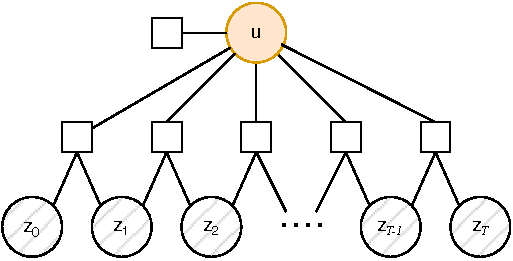
\includegraphics{FG_ts.drawio.pdf}
    \caption{Factor graph  for the generating equations of \eqref{eq:ts-sem}}
    \label{fig:ts_fg}
\end{figure}

% \subsection{Noisy observations}
% For exposition in this paper, we have assumed that we observe realisations of the series noiselessly.
% More generally, we might observe some noisy linear function of the true target values.
% \begin{align*}
%     \state_{t}&=\op{P}(\state_{\tm}, \forcing),\quad t=1, 2, \cdots, T\\
%     \outp_{t}&=\op{Y}\state_{t},\quad t=1, 2, \cdots, T\numberthis\label{eq:ts-sem-noisy}
% \end{align*}\nb{missing priors}
% where our observations are actually of \(\outp_{t}=\outpst_{t}\).
% Then the associated factor graph is more complicated (Figure~\ref{fig:ts_fg_noisy}) and the inference procedure is in fact loopy belief propagation.
% In this case we need to solve the filtering problem, estimating \(\{\state_{t}\}_t\) from \(\{\outp_{t}\}_t\).
% The message-pasing schedule in this case is loopy, and may not converge, although the ensemble updates are well-defined under the assumption that our ensemble statistics are.
% \begin{figure}
%     \centering
%     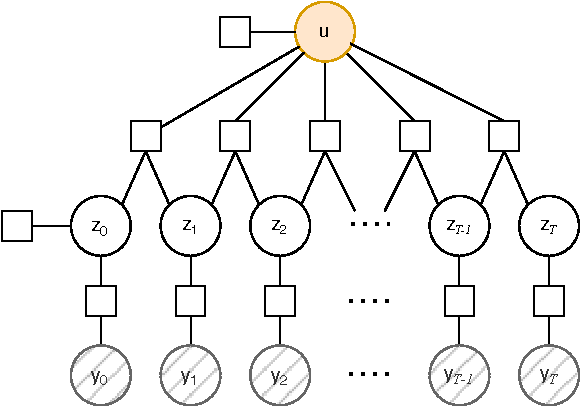
\includegraphics{FG_ts_noisy.drawio.pdf}
%     \caption{Factor graph for the generating equations of \eqref{eq:ts-sem-noisy}}
%     \label{fig:ts_fg_noisy}
% \end{figure}

% \section{Stationary moves in an ensemble Gaussian posterior}
% \subsection{Elliptical slice sampling}
% \subsection{Langevin}
% Suppose \(\vrv{x}\) is a  \(d\)-dimensional Gaussian RV 
% \begin{align*}
% \vrv{x}&\sim\mathcal{N}(\overline{m}_{x}, \mm{K}_{\vrv{x}\vrv{x}})
% \end{align*}
% whose moments are  chosen to match the empirical moments of an ensemble \(\mm{X}=\begin{bmatrix}
%     \vrv{x}^{(1)} & \cdots & \vrv{x}^{(N)}
% \end{bmatrix}\) of iid samples
% so that
% \begin{align*}
% \overline{m}_{\vrv{x}}&:=\frac{1}{N}\sum_{i=1}^N \tilde{\vrv{x}^{(i)}}\\
% \mm{K}_{\vrv{x}\vrv{x}} &:= \breve{\mm{X}} \breve{\mm{X}}^{\top}\\
% \breve{\mm{X}}&=\frac{1}{\sqrt{N-1}}\begin{bmatrix}
%     (\vrv{x}^{(1)}-\overline{m}_{\vrv{x}}) & \cdots & (\vrv{x}^{(N)}-\overline{m}_{\vrv{x}})
% \end{bmatrix}\\
% \end{align*}
% Note that that the deviation matrix represents a square-root factorisation for the covariance, we can simulate new realisations from the distribution of this variable using
% \(\rv{x}\sim{m}_{\vrv{x}} + \breve{\mm{X}}\xi\) for \(\xi\sim\mathcal{N}(\vv{0}, \mm{I})\).
% A corollary to this is that this distribution and its updates comprise linear combinations of members of the ensemble, and so if \(d>N\) it cannot span the space of all possible realisations.\nb{not quite. what does it actually imply?}

% We could diversify the ensemble, in the sense of simulating realisations with the same moments but which did not come from the span of the ensemble if there existed a non-trivial random transform \(j\) which was not restricted to the span of this basis such that \(\vrv{x}\sim \dist{N}({m}_{\vrv{x}},\mm{K}_{\vrv{x}})\Rightarrow j(\vrv{x}) \disteq \vrv{x}\).
% Can we construct such a \(j\)?

% Langevin dynamics might be a tractable approach.
% Given \(\vrv{z}\sim\mathcal{N}(0,\mm{I}_{d})\) and a step size \(\epsilon\), an Euler-Maruyama approximation to a Langevin move is
% \begin{align*}
% j(\vv{x})
% &:= \vv{x}
% + \epsilon \nabla_{\vv{x}} \log p_{\vrv{x}}(\vv{x}) 
% + \sqrt{2\epsilon}~\vrv{z},\text{ and}\\
% \nabla_{\vv{x}} \log p_{\vrv{x}}(\vv{x})
% &=-( \vv{x}-{m}_{\vrv{x}})^{\top}\mm{K}_{\vrv{x}\vrv{x}}^{-1}
% \end{align*}
% thus
% \begin{align*}
% \Delta\vv{x} - \sqrt{2\epsilon}~ \vrv{z}
% &=\epsilon ( \vv{x}-{m}_{\vrv{x}})^{\top}\mm{K}_{\vrv{x}\vrv{x}}^{-1} \\
% (\Delta\vv{x} - \sqrt{2\epsilon}~ \vrv{z})\mm{K}_{\vrv{x}\vrv{x}}
% &=\epsilon ( \vv{x}-{m}_{\vrv{x}})^{\top}.
% \end{align*}
% Can we find any cool simplifications by plugging in ensemble deviations?
% Let us try:
% \begin{align*}
% \Delta\vv{x} - \sqrt{2\epsilon}~ \vrv{z}
% &=\epsilon ( \vv{x}-{m}_{\vrv{x}})^{\top}(\breve{\mm{X}} \breve{\mm{X}}^{\top})^{-1} \\
% (\Delta\vv{x} - \sqrt{2\epsilon}~ \vrv{z})\breve{\mm{X}} \breve{\mm{X}}^{\top}
% &=\epsilon ( \vv{x}-{m}_{\vrv{x}})^{\top} \\
% \Delta\vv{x} 
% &=\epsilon ( \vv{x}-{m}_{\vrv{x}})^{\top}(\breve{\mm{X}} \breve{\mm{X}}^{\top})^{-1} + \sqrt{2\epsilon}~ \vrv{z}
% \end{align*}
% We can batch this, in which case
% \begin{align*}
% \Delta\mm{X} 
% &=\epsilon (N-1) \breve{\mm{X}}^{\top}(\breve{\mm{X}} \breve{\mm{X}}^{\top})^{-1} + \sqrt{2\epsilon}~ \vrv{Z}\\
% \Delta\mm{X}  - \sqrt{2\epsilon}~ \vrv{Z} &=\epsilon (N-1) \breve{\mm{X}}^{\top}(\breve{\mm{X}} \breve{\mm{X}}^{\top})^{-1} 
% \end{align*}

% This Euler-Maruyama approximation will clearly be bad if \(\epsilon\) is not tiny; we could consider implicit steps or Metropolis adjustment?
% Both those look expensive.

% We expect that iterating such steps will not be truly stationary; in the end the posterior covariance will drift.

% \section{Epistemic uncertainty in the ensemble posterior}\label{sec:u-uncertainty}

% Consider a jointly Gaussian ensemble covariance which includes a term to inflate the uncertainty of  our estimate of the posterior, because, e.g., we would like to decrease the confidence of our estimate convinced that it is \emph{truly} Gaussian, and quantifying that by adding Gaussian noise is the laziest option that might work.
% (Student-t distributions look hard and boring).
% This model looks similar to \eqref{eq:discrete_joint_enkf_sim} but with the uncertainty term moved:
% \begin{align*}
% \left.\left[\begin{array}{c}
%     \state_{t} \\
%     \forcing
% \end{array}\right]\right|\state_{\tm}
% &\simeq\dist{N}\left(
%     \left[\begin{array}{c}
%         \overline{\statest}\\
%         \overline{\forcingst}
%     \end{array}\right],
%     \left[\begin{array}{cc}
%         \breve{\mm{Z}}\breve{\mm{Z}}^{\top} 
%         & \breve{\mm{U}}\breve{\mm{Z}}^{\top} \\\ % 3 backslashes or it breaks for some reason
%         \breve{\mm{Z}}\breve{\mm{U}}^{\top}
%         & \breve{\mm{U}}\breve{\mm{U}}^{\top} +\mm{K}_{\xi}
%     \end{array}\right]\numberthis\label{eq:discrete_joint_enkf_sim_misfit}
% \right).
% \end{align*}
% % What does that look like in ensemble inference?

% % \subsection{Adding independent noise to the samples}

% Simplest options:
% We can add some noise to each of the samples \(\forcingst^{(i)}\gets\vrv{\xi}^{(i)}\sim\mathcal{N}(0,\mm{K}_{\xi}).\)
% Is this well posed?
% How about if \(\mm{K}_{\xi}=\tau^2\mm{I}\)?
% Connection to Langevin sampling above.

% \subsection{Inflating posterior covariance}

% According to \citep{RothEnsemble2017} this is called variance inflation and is discussed in the literature.

% Alternatively, suppose the posterior ensemble has covariance  \(\breve{\mm{U}}\breve{\mm{U}}^{\top}\) but we wish it had covariance \(\breve{\mm{U}}'\breve{\mm{U}}'{}^{\top} \succ\breve{\mm{U}}\breve{\mm{U}}^{\top}\).
% 
% We could change that by scaling the ensemble, possibly randomly, about the mean by some scalar (?) inflation factor \(\rv{s}\), \(\Ex\rv{s}>1\),
% \(\forcingst^{(i)}\gets\rv{s}(\forcingst^{(i)}-m_{\forcing})\) or even 
% \(\forcingst^{(i)}\gets\vrv{S}(\forcingst^{(i)}-m_{\forcing})\) from some matrix-valued \(\vrv{S}\).

% Hmm, products of RVs is a complicated world to be in; I think I vote for deterministic scaling, or additive Gaussian noise, now that I think about it.

% \section{Ensemble Bayesian inversion 1: by pathwise GP sampling and error propagation}
% Here is a bad way of solving this problem because NN people always need to try the Jacobian first.

% Rather than assuming a jointly Gaussian distribution for all variables as in \eqref{eq:gaussian_approx_proc}, we make the weaker assumption that \emph{conditional on some fixed sample \(\state_{\tm}{=}\statest_{\tm}\), \(\state_{t}{=}\statest_{t}\) and \(\forcing\)} are jointly Gaussian with a conditional variance given by a local first-order Taylor expansion about \(\forcing{=}\forcingst\).
% That is, at pair \((\forcing, \state_{\tm})=(\forcingst, \statest_{\tm})\), the linearised joint distribution is
% \begin{align*}
%     {m}_{\forcing}
%         &=\proj_{\vv{X}}\forcing \numberthis\label{eq:mvn-m-inp}\\
%     {m}_{\state_{t}}
%         &=\proj_{\vv{S}}[\op{P}(\statest_{\tm},\forcingst)]\numberthis\label{eq:mvn-m-state}\\
%     \mm{K}_{\state_{t}\state_{t}}
%          &=J_{\forcingst}\mm{K}_{\forcing\forcing}J_{\forcingst}^{\top} +\sigma^2\mm{I}\numberthis \label{eq:discrete_pred_cov_taylor_local}\\
%     \mm{K}_{\state_{t}\forcing}
%     %     &= [\vv{k}_{\state_{t}\forcing}(s_i,x_j)]_{ij} \\
%     % \mm{K}_{\statest\forcingst}{}
%         &=\mm{K}_{\forcing\forcing}J_{\forcingst}^{\top}\numberthis 
% \end{align*}
% where \(J_{\forcingst}:=\nabla_{\forcingst'}\proj_{\vv{S}}\op{P}(\statest_{\tm},\forcingst)\in\mathbb{R}^{|S|}\times\mathbb{R}^{|X|}\) is the Jacobian matrix of the projection of the forward predictor at this point.
% This rule gives us a different update \emph{for each sample} based on a different local linearisation.

% The Matheron update analog to \eqref{eq:pathwise-update} in such a model is thus
% \begin{align*}
% &(\tilde{{\forcing}} \gvn \state_{t}{=}\statest_{t},\state_{\tm}) \\
% &\disteq 
% \tilde{{\forcing}}+\mm{K}_{\state_{t}\forcing} \mm{K}_{\state_{t}\state_{t}}^{-1}\left(\statest_{t}-{m}_{\state_{t}}\right)\\
% &=\tilde{{\forcing}}+\mm{K}_{\forcing\forcing}J_{\forcingst}^{\top} (J_{\forcingst}\mm{K}_{\forcing\forcing}J_{\forcingst}^{\top} +\sigma^2\mm{I})^{-1}\left(\statest_{t}-{m}_{\state_{t}}\right).\numberthis\label{pathwise-update-mc}
% \end{align*}
% This method has various apparent difficulties.
% % For one, the matrix inversion required by the update step \eqref{eq:pathwise-update} is an \(\mathcal{O}(|X||S|^3)\) operation.
% Under the discretisation \eqref{eq:discrete_joint_naive}, calculating the update \eqref{eq:discrete_pred_cov_taylor_local} naively is a \(\mathcal{O}(|X|^3|S|)\) operation since we need to invert  \(\mm{K}_{\forcing\forcing})\) to calculate it.
% Although this method has relaxed some assumptions of the Gaussian variational posterior approximation, it is even less computationally tractable; each sample update requires both the covariance inversion and the calculation of a different local Jacobian matrix.

% Ensemble Kalman methods~\cite{EvensenData2009} empirically approximate intractably large covariance matrices \(\mm{K}_{\forcing\forcing}\), e.g.\ in \eqref{eq:pathwise-update} where we need to find an update.

% Then,
% \begin{align*}
% &\mm{K}_{\forcing\forcing}J_{\forcingst}^{\top} (
%     J_{\forcingst}\mm{K}_{\forcing\forcing}J_{\forcingst}^{\top}
%     +\sigma^2\mm{I}
%     )^{-1}\\
% % &=\frac{1}{\sigma^2}(
% %     \mm{K}_{\forcing\forcing}^{-1} + \frac{1}{\sigma^2} J_{\forcingst}^{\top}J_{\forcingst}
% %     )^{-1}J_{\forcingst}^{\top}\\
% &\simeq\breve{\mm{U}}\breve{\mm{U}}^{\top}J_{\forcingst}^{\top} (
%     J_{\forcingst}\breve{\mm{U}}\breve{\mm{U}}^{\top}J_{\forcingst}^{\top}
%     +\sigma^2\mm{I}
%     )^{-1}\\
% &=\underbrace{\breve{\mm{U}}}_{|X|\times N} \left(
%         \underbrace{\breve{\mm{U}}^{\top}}_{N\times |X|}
%         \underbrace{J_{\forcingst}^{\top}}_{|X|\times |S|}
%         \underbrace{J_{\forcingst}}_{|S|\times |X|}
%         \underbrace{\breve{\mm{U}}}_{|X|\times N}
%         +\frac{1}{\sigma^2}\mm{I}
%     \right)^{-1}
%     \underbrace{\breve{\mm{U}}^{\top}}_{N\times |X|}
%     \underbrace{J_{\forcingst}^{\top}}_{|X|\times |S|}
% \end{align*}
% Another useful one is the Kalman gain,
% \begin{align*}
% \mm{G} &:=\mm{K}_{\forcing\forcing}J_{\forcingst}^{\top} (J_{\forcingst}\mm{K}_{\forcing\forcing}J_{\forcingst}^{\top} +\sigma^2\mm{I})^{-1}\\
% \underbrace{\mm{G}}_{|X|\times |S|} &:=
%     \underbrace{\breve{\mm{U}}}_{|X|\times N}
%     \underbrace{J_{\forcingst}^{\top}}_{|X|\times |S|}
%     \left(
%         \underbrace{J_{\forcingst}}_{|S|\times |X|}
%         \underbrace{\breve{\mm{U}}}_{|X|\times N}
%         \underbrace{\breve{\mm{U}}^{\top}}_{N \times |X|}
%         \underbrace{J_{\forcingst}^{\top}}_{|X| \times |S|}
%         +\sigma^2\mm{I}
%     \right)^{-1}
% \end{align*}
% which we can calculate by solving for
% \begin{align*}
% \mm{G}\left(J_{\forcingst}\breve{\mm{U}}\breve{\mm{U}}^{\top}J_{\forcingst}^{\top} +\sigma^2\mm{I}\right) &:=\breve{\mm{U}}\breve{\mm{U}}^{\top} J_{\forcingst}^{\top}
% \end{align*}
% % or using Welling's variant Woodbury:
% % If \(\mathbf{P}, \mathbf{R}\) are positive definite, then
% % \begin{align*}
% %     \mathbf{P} \mathbf{B}^{\top}\left(\mathbf{B} \mathbf{P} \mathbf{B}^{\top}+\mathbf{R}\right)^{-1}
% %     =\left(\mathbf{P}^{-1}+\mathbf{B}^{\top} \mathbf{R}^{-1} \mathbf{B}\right)^{-1} \mathbf{B}^{\top} \mathbf{R}^{-1}
% % \end{align*} from which
% % \begin{align*}
% %     &(\breve{\mm{U}}^{\top}\breve{\mm{U}}) J_{\forcingst}^{\top}\left(J_{\forcingst} (\breve{\mm{U}}^{\top}\breve{\mm{U}}) J_{\forcingst}^{\top}+(\sigma^2\mm{I})\right)^{-1}\\
% %     &=\frac{1}{\sigma^2}\left((\breve{\mm{U}}^{\top}\breve{\mm{U}})^{-1}+\frac{1}{\sigma^2}J_{\forcingst}^{\top}  J_{\forcingst}\right)^{-1} J_{\forcingst}^{\top} 
% % \end{align*}
% which is not \emph{prima facie} a huge saving, although we can group the \(\underbrace{J_{\forcingst}}_{|S|\times |X|}\underbrace{\breve{\mm{U}}}_{|X|\times N}\) terms.

% \section{Design}
% a.k.a. choosing projections.

% We largely ignore the question of optimal placement of observation in the current work.
% Optimal \(\set{S}\)~\cite{AlexanderianOptimal2021}?
% Optimal \(\Phi\)~\cite{LassasDiscretizationinvariant2009}? 

% What do we actually converge to if we try to update th whole thing using low-dim projections?

% The unfavourable scaling is in the output observation term, so we now have a question about how big to make that. There are some results in subsampling covariance observations that we possibly need to digest to manage this term \cite{ChenStochastic2020,MinhFinite2022}.

% \section{Offcut: Posterior updates by random projections}

% Can we make site updates of posterior fields cheaper by updating random projections of the field in some sense?

% As seen in sliced Fisher score matching.
% Is that a way of doing partial updates?

% \section{Offcut: inversion by Newton methods}
% \cite{WilkinsonBayesNewton2021}

% \subsubsection{by that weird Laplace-on-a-graph trick the opposition uses}
% \cite{MagnaniApproximate2022}  

% \subsection{Robust losses}

% \cite{DavisonFutureMapping2019,DonohoHigh2013}
\fi
